% TODO: images are on counted
\section{ЗАДАЧА МАРКЕТИНГОВОЇ РОЗВІДКИ}
% Ми не створюємо канал як такий. Метою роботи є маркетингове прогнозування 
% шляхом моделювання маркетингового каналу.
%
% TODO: можливо, заголовок треба буде змінити
% TODO: додати новий сорець
\subsection{Огляд проблем МІС}
\subsubsection{Основні поняття}
\subsubsection{Маркетингова розвідка як складова МІС}
% подчеркнуть разведку в міс
% абзац
\begin{stdfigure}
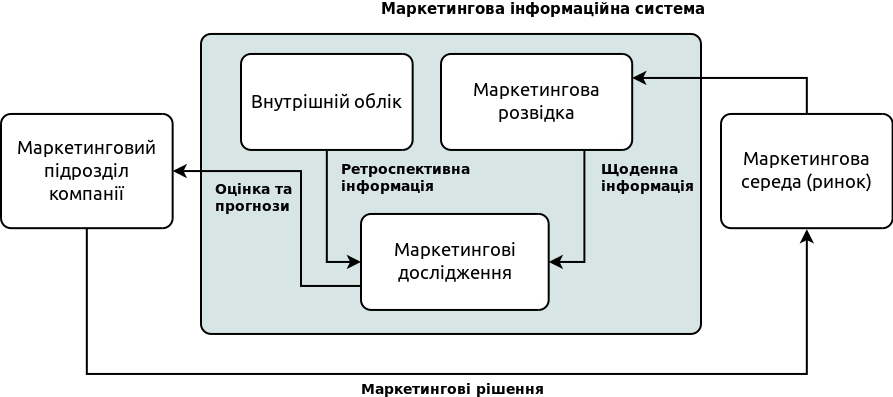
\includegraphics[width=7in]{images/mis_structure.png}
\caption{Структура МІС}
\label{fig:mis_structure}
\end{stdfigure}    

\subsubsection{Компоненти підсистеми маркетингової розвідки}

\subsection{Бізнес-ігри}
\subsubsection{Поняття бізнес-гри}

\subsubsection{Моделювання маркетингових каналів}
%    MIS складається з трьох частин:

\subsubsection{Постановка задачі моделювання}

\subsection{Вимоги до ПЗ}
\subsubsection{Функціональні вимоги}
%TODO: use case, idef0

\subsubsection{Нефункціональні вимоги}
% 6 критеріїв ISO 
\subsection{Завдання на розробку ПЗ}
